\chapter{推論統計：區間估計}

    統計中對於未知參數的估計方法有兩種：\textit{點估計} (point estimation) 和\textit{區間估計} (interval estimation)。點估計較為直觀，即利用樣本求出一個統計量（稱為估計量）來估計未知參數。我們在第二章已經提到針對母體平均與母體變異數的最佳點估計量（即樣本平均與樣本變異數），並在第五章中提到評估點估計量時需要知道估計量的抽樣分布，以了解該估計量是否為不偏估計量、以及該估計量的標準誤多大。

    \medskip
    
    本章我們將會深入探討參數的另一類估計方法：區間估計。我們將從母體平均的區間估計建構方式出發，了解樣本平均的抽樣分布在區間估計扮演的角色，以及如何正確解釋區間估計隱含的機率敘述。最後，我們會介紹一個在建構信賴區間與後續假說檢定都至關重要的連續型分布：\textit{t} 分布 (\textit{t} distribution)。
    
    \begin{introduction}[第 \thechapter 章學習目標]{1}
        \item 了解估計的兩種型式：點估計和區間估計
        \item 了解如何用機率語言解釋信賴區間的意義
        \item $t$ 分布的由來以及與標準常態分布的關係
        \item 母體為常態分布下母體平均信賴區間的建構方法
        \item 母體為其他分布下母體平均信賴區間的建構方法
    \end{introduction}

    點估計是用一個數值來估計母體參數，因此我們需要額外用估計值的標準誤來量化點估計的不確定性。區間估計則是利用區間來估計參數，例如「我們有 95\% 的信心，清華大學生的平均身高將被 (160, 170) 公分這個區間覆蓋。」這樣的估計方法雖然沒有明確指出一個估計值，但是同時告知了參數的約略位置以及估計的不確定性，因此被稱為區間估計。

    \medskip
    
    建構區間估計的其中一種方法是先尋找一個含未知參數、但分布已知的量（這在統計中被稱為樞紐量 (pivotal quantity)）。舉例來說，假設我們已知清華大學生的身高呈現常態分布且標準差為 5 公分，但是不知道平均值為何。若把這個未知的母體平均設為 $\mu$ 公分，則身高 $X$ 的分布可寫為：
    \smallskip
    \[X \sim \NN(\mu, 5^2)\]
    \smallskip
    為了估計 $\mu$，假設我們抽了 36 位學生測量身高，並將平均身高記為 $\bar{X}$ 公分。由於 $\bar{X}$ 為樣本平均，根據常態分布的性質，其抽樣分布亦為常態分布，可寫為：
    \smallskip
    \[\bar{X} \sim \NN\Big(\mu, \frac{5^2}{36}\Big)\]
    \smallskip
    此時將 $\bar{X}$ 作 $z$ 分數轉換，就可以得到一個服從標準常態分布的量：
    \smallskip
    \[\frac{\bar{X} - \mu}{5/\sqrt{36}} \sim \ZZ\]
    \smallskip
    注意到這個量含有未知參數 $\mu$，但其分布卻是已知，因此它是一個樞紐量。此時如果我們想得到具有 $95\%$ 信心的區間估計，可以先根據定義，為樞紐量的分布（這裡是標準常態分布）建構出一個以 $0$ 為中心、左右對稱、且機率為 $95\%$ 的區間：
    \smallskip
    \[\PP(-z_{0.025} < \ZZ < z_{0.025}) = 1-2 \times 0.025 = 0.95\]
    \smallskip
    此處 $z_{0.025}$ 是已知的數值，查 Z 表可得到大約是\textbf{1.96}。由此我們可以推出：
    \smallskip
    \begin{align*}
        \PP\Big(-z_{0.025} < \frac{\bar{X} - \mu}{5/\sqrt{36}} < z_{0.025}\Big) &= 0.95\\
        \PP\Big(-z_{0.025}\cdot \frac{5}{\sqrt{36}} < \bar{X} - \mu < z_{0.025}\cdot \frac{5}{\sqrt{36}}\Big) &= 0.95\\
        \PP\Big(\bar{X}-z_{0.025}\cdot \frac{5}{\sqrt{36}} < \mu < \bar{X} + z_{0.025}\cdot \frac{5}{\sqrt{36}}\Big) &= 0.95\\
        \PP\Big(\mu \in \Big(\bar{X}-z_{0.025}\cdot \frac{5}{\sqrt{36}},  \bar{X} + z_{0.025}\cdot \frac{5}{\sqrt{36}}\Big)\Big) &= 0.95
    \end{align*}
    \smallskip
    上述的式子代表，在母體服從 $\NN(\mu, 5^2)$ 的假設下，如果我們不斷抽取 36 位學生，並把每次得到的平均身高 $\bar{X}$ 都拿來算出一個區間 $\big(\bar{X}-z_{0.025}\cdot \frac{5}{\sqrt{36}},  \bar{X} + z_{0.025}\cdot \frac{5}{\sqrt{36}}\big)$，那麼這個區間覆蓋到 $\mu$ 的機率為 $95\%$。以圖\ref{fig:confidence_interval}為例，當$\mu = 160$時，重複抽取 36 人 200 次得到的 200 個區間中，僅有 10 個未蓋到 $160$ （在圖中以紅色標示），即蓋到的機率為 $190/200 = 95\%$。區間計算方式滿足上述性質時，我們稱\textbf{$\big(\bar{X}-z_{0.025}\cdot \frac{5}{\sqrt{36}},  \bar{X} + z_{0.025}\cdot \frac{5}{\sqrt{36}}\big)$是$\mu$ 的 95\% 信賴區間}。而因為這個信賴區間同時具有上下限，我們也常稱這種信賴區間為\textit{雙尾信賴區間}。
    
    \begin{figure}[htbp]
        \centering
        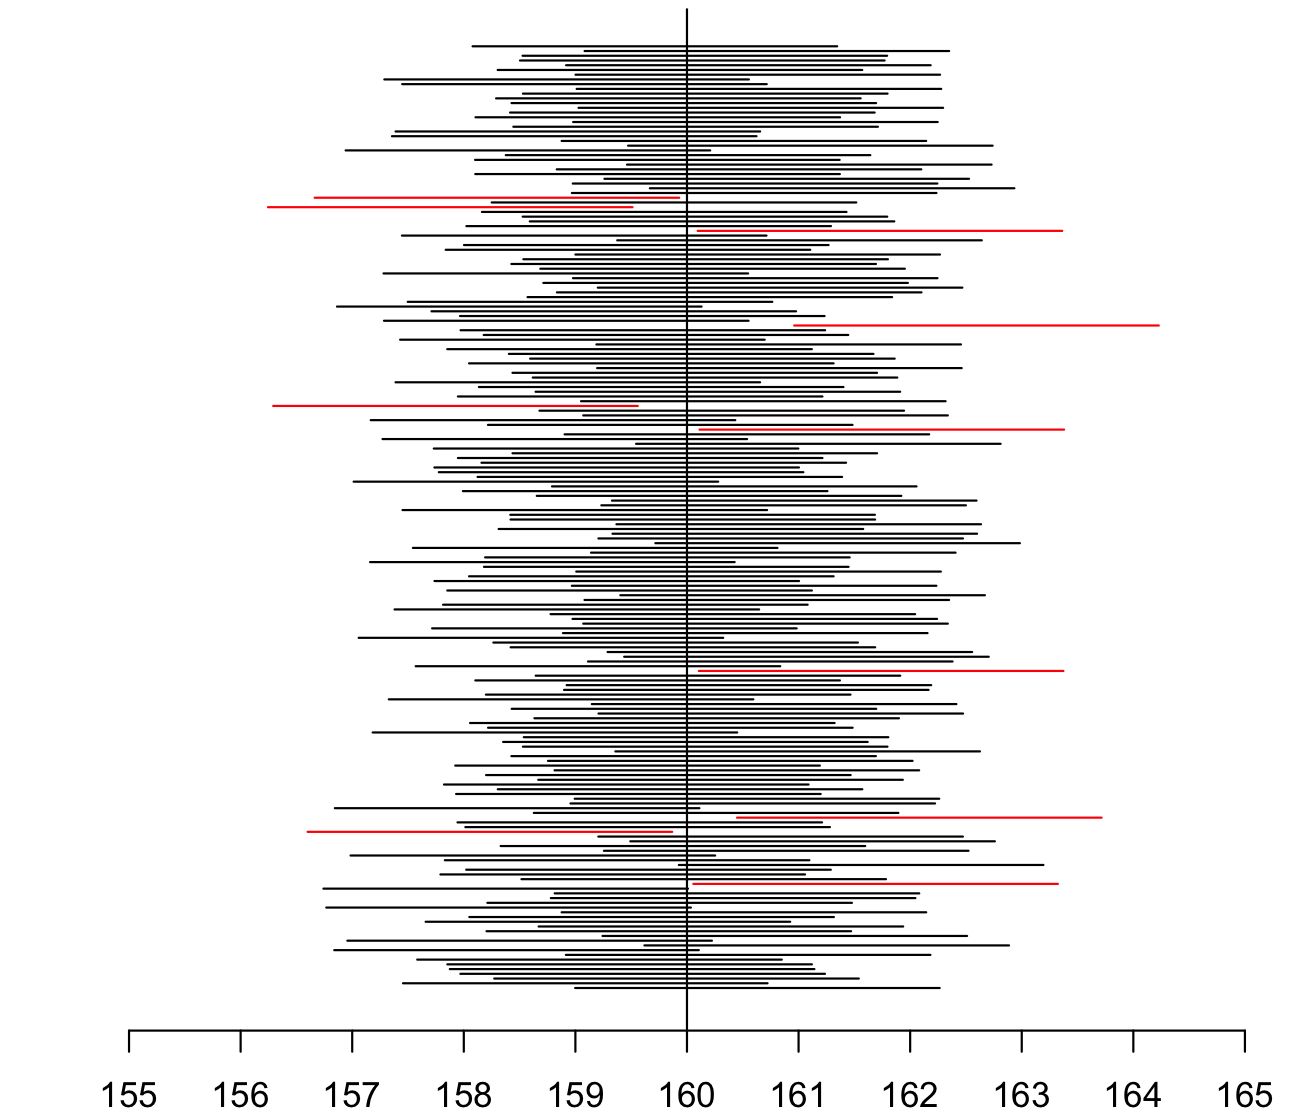
\includegraphics[width=0.8\textwidth]{figures/06-Confidence_interval/Confidence_interval.png}
        \caption{從 $\NN(160, 5^2)$ 抽出樣本數 36 的 200 組樣本，所得到的200個平均值 95\% 信賴區間}
        \label{fig:confidence_interval}
    \end{figure}
    
    注意到上述信賴區間性質的定義中，隨著每次抽樣，$\bar{X}$會有所變動，因此\textbf{整個區間會隨著抽樣而有不確定性}。這個「區間具有不確定性」的觀念可以衍生出兩個重點：
    \begin{itemize}
        \item \underline{信賴區間的機率是針對「產生信賴區間的算法」而非觀察到的信賴區間數值}：\\我們抽得一個樣本後，可以根據該樣本的觀察值算出一個區間（即圖 \ref{fig:confidence_interval}中的其中一條橫線）。但這個區間只是眾多可能的區間中被抽樣出來的一個，而信賴區間裡的 $95\%$ 是針對整體可能的區間作的機率性描述，而不是針對單一的區間觀察值。
        \item \underline{參數雖未知但不具變動性，區間才有抽樣造成的變動性}：\\前面我們在描述 $\PP\big(\mu \in \big(\bar{X}-z_{0.025}\cdot \frac{5}{6},  \bar{X} + z_{0.025}\cdot \frac{5}{6}\big)\big)$ 時，不用 $\mu$ 「落在」區間的機率，而是用區間「覆蓋」$\mu$ 的機率，即為強調 $\mu$ 本身不動，是區間在隨著抽樣而變動的概念。
    \end{itemize}

    \medskip
    
    前面我們用了一些實際數字來演示信賴區間的建構方法。若利用符號作一般性推導，假設母體來自於已知標準差為 $\sigma$ 的常態分布，且 $\bar{X}$ 為樣本數 $n$ 的樣本得出之樣本平均，則母體平均值的 $(1-\alpha) \times 100\%$ 雙尾信賴區間可寫為
    \smallskip
    \[\Big(\bar{X}-z_{\alpha/2}\frac{\sigma}{\sqrt{n}},  \bar{X} + z_{\alpha/2}\frac{\sigma}{\sqrt{n}}\Big)\]
    \smallskip
    可以看到，這個雙尾區間以樣本平均 $\bar{X}$ 為中心，左右的寬度則各為 $z_{\alpha/2}\frac{\sigma}{\sqrt{n}}$。寬度取決於三個因子，其變動方向與寬度變動的關係均十分直觀合理：
    \begin{itemize}
        \item 母體標準差 $\sigma$：母體標準差越大，代表每一個觀察值帶有的雜訊越多，因而估計的不確定度變高，信賴區間寬度變寬。
        \item 樣本數 $n$：樣本數越大，針對母體平均的資訊越多，因而能估計得越精準，信賴區間寬度變窄。
        \item 信賴區間的覆蓋率 $1-\alpha$：要使信賴區間的覆蓋率拉高，就應該要把信賴區間拉寬以減少覆蓋不到真實母體平均的機率。從公式來看，覆蓋率越高，$\alpha$越小，$z_{\alpha/2}$的值就越大，使得信賴區間的寬度變寬。
    \end{itemize}
    %上面我們探討的是雙尾區間。若我們有興趣的是單尾的信賴區間，則可以利用 $\PP(\ZZ > -z_{\alpha}) = \PP(\ZZ < z_{\alpha}) = 1-\alpha$ ，以相同的推導方式建立出下列右尾和左尾$(1-\alpha) \times 100\%$信賴區間：
    %\[\Big(\bar{X}-z_{\alpha}\frac{\sigma}{\sqrt{n}},  \infty\Big), \;\;\Big(-\infty,  \bar{X} + z_{\alpha}\frac{\sigma}{\sqrt{n}}\Big)\]

    \bigskip

    \begin{custom}{動手作}
       假設已知 60 歲以上國人血清低密度脂蛋白的濃度標準差為 10 mg/dL，且呈現常態分布。現隨機選取 400 位 60 歲以上的志願者抽血，得到血清低密度脂蛋白的平均濃度為 93 mg/dL。請問 60 歲以上國人平均血清低密度脂蛋白濃度的95\%、90\% 與 100 \% 雙尾信賴區間為何？
    \end{custom}

    \answerbox{200pt}

    \bigskip

    \begin{custom}{動動腦}
        我們在前面推導 $95\%$ 信賴區間時，先針對標準常態分布建立了一個對稱於 $0$ 、機率恰為 $95\%$ 的區間 $(-z_{0.025}, z_{0.025})$。如果不要求該區間對稱於 $0$，是否還有其他符合機率的區間？這些區間對應的信賴區間會是什麼形式？如果允許該區間沒有上界或沒有下界，對應的信賴區間會變成什麼形式？在所有雙尾信賴區間（有上下界的信賴區間）中，為什麼會預設使用「相對於樣本平均對稱」的建構方法？
    \end{custom}

    \answerbox{350pt}

    \bigskip

    若母體並非來自常態分布，平均值信賴區間的建構較不直觀。然而，當樣本數夠大時，我們還有一個重要的法寶：中央極限定理！舉例來說，在前一章我們提到了民調詢問支持率的例子：如果把每個人支持與否紀錄為 $1$ 和 $0$，那麼每個人的回答就來自於機率參數為支持率 $p$ 的白努利分布，而 $n$ 位受訪者的經驗支持率 $\hat{p}$ 相當於從該白努力分布抽取樣本數為 $n$ 的樣本而算出的樣本平均。根據中央極限定理：
    \smallskip
    \[\hat{p} \leadsto \NN\Big(p, \frac{p(1-p)}{n}\Big)\]
    \smallskip
    所以利用類似常態分布的方法，我們可以構造以下關於 $p$ 的（近似） $(1-\alpha)\times 100\%$雙尾信賴區間
    \smallskip
    \[\Big(\hat{p} - z_{\alpha/2} \sqrt{\frac{p(1-p)}{n}}, \hat{p} + z_{\alpha/2} \sqrt{\frac{p(1-p)}{n}}\Big)\]
    \smallskip
    不過上面式子的問題是，根號中的 $p$ 仍是未知的參數，所以我們用 $p$ 最好的估計值 $\hat{p}$ 來取代 $p$，最終得到
    \smallskip
    \[\Big(\hat{p} - z_{\alpha/2} \sqrt{\frac{\hat{p}(1-\hat{p})}{n}}, \hat{p} + z_{\alpha/2} \sqrt{\frac{\hat{p}(1-\hat{p})}{n}}\Big)\]
    \smallskip
    這個公式也常被當成是比例信賴區間的通式。同樣地，右尾和左尾的（近似） $(1-\alpha)\times 100\%$單尾信賴區間為
    \smallskip
    \[\Big(\hat{p} - z_{\alpha} \sqrt{\frac{\hat{p}(1-\hat{p})}{n}}, 1\Big), \;\; \Big(0, \hat{p} + z_{\alpha} \sqrt{\frac{\hat{p}(1-\hat{p})}{n}}\Big)\]
    \smallskip
    此處左右尾的界線設定在 0 和 1，因為實際上的參數 $p$ 不可能超過 $[0,1]$ 的範圍。注意到這些近似信賴區間只有在 $n$ 夠大的時候，聲稱的 $(1-\alpha)\times 100\%$ 覆蓋率才會成立。一般而言，當 $np$ 及 $n(1-p)$ 均大於 $5$ 時，這個信賴區間的表現就已經很不錯。

    \bigskip
    
    \begin{custom}{動手作}
        某大型醫療體系對員工進行血糖抽檢，隨機抽檢 160 人後發現，有 12 員工呈現空腹血糖過高的現象。請問該體系員工空腹血糖過高比率之 95\% 信賴區間為何？
    \end{custom}

    \answerbox{180pt}

    \bigskip

    \begin{custom}{動手作}
        某民調公司希望藉由隨機電訪了解民眾對於 A 總統的支持度。若民調公司希望無論調查結果如何，最後建構出之支持度 95\% 雙尾信賴區間均不寬於上下 3\% （也就是總寬度不超過 6\%），且暫不考慮拒答的問題，那麼至少應收回多少有效電訪樣本？
    \end{custom}

    \answerbox{220pt}

    \bigskip

    前面我們針對常態分布的母體平均建立信賴區間時，作了一個不太常見的假設：母體標準差已知。大部分的情況下，母體標準差都是未知的，因此雙尾信賴區間的公式就會多出一個未知數 $\sigma$。最直覺的解決辦法是直接參考比例信賴區間的做法，用樣本標準差帶入 $\sigma$。然而，這個方法在 $n$ 不夠大時，樣本標準差估計的準確度不佳，會造成整體的信賴區間覆蓋率不足。舉例來說，圖\ref{fig:confidence_t}中，假設母體和圖\ref{fig:confidence_interval}一樣服從 $\NN(160, 5^2)$，但是樣本數只有 9，且我們使用前述的雙尾 95\% 信賴區間公式並把 $\sigma$ 帶入樣本標準差，則 200 個平均值信賴區間中，有高達 18 個沒有覆蓋到正確值 160！

    \begin{figure}[htbp]
        \centering
        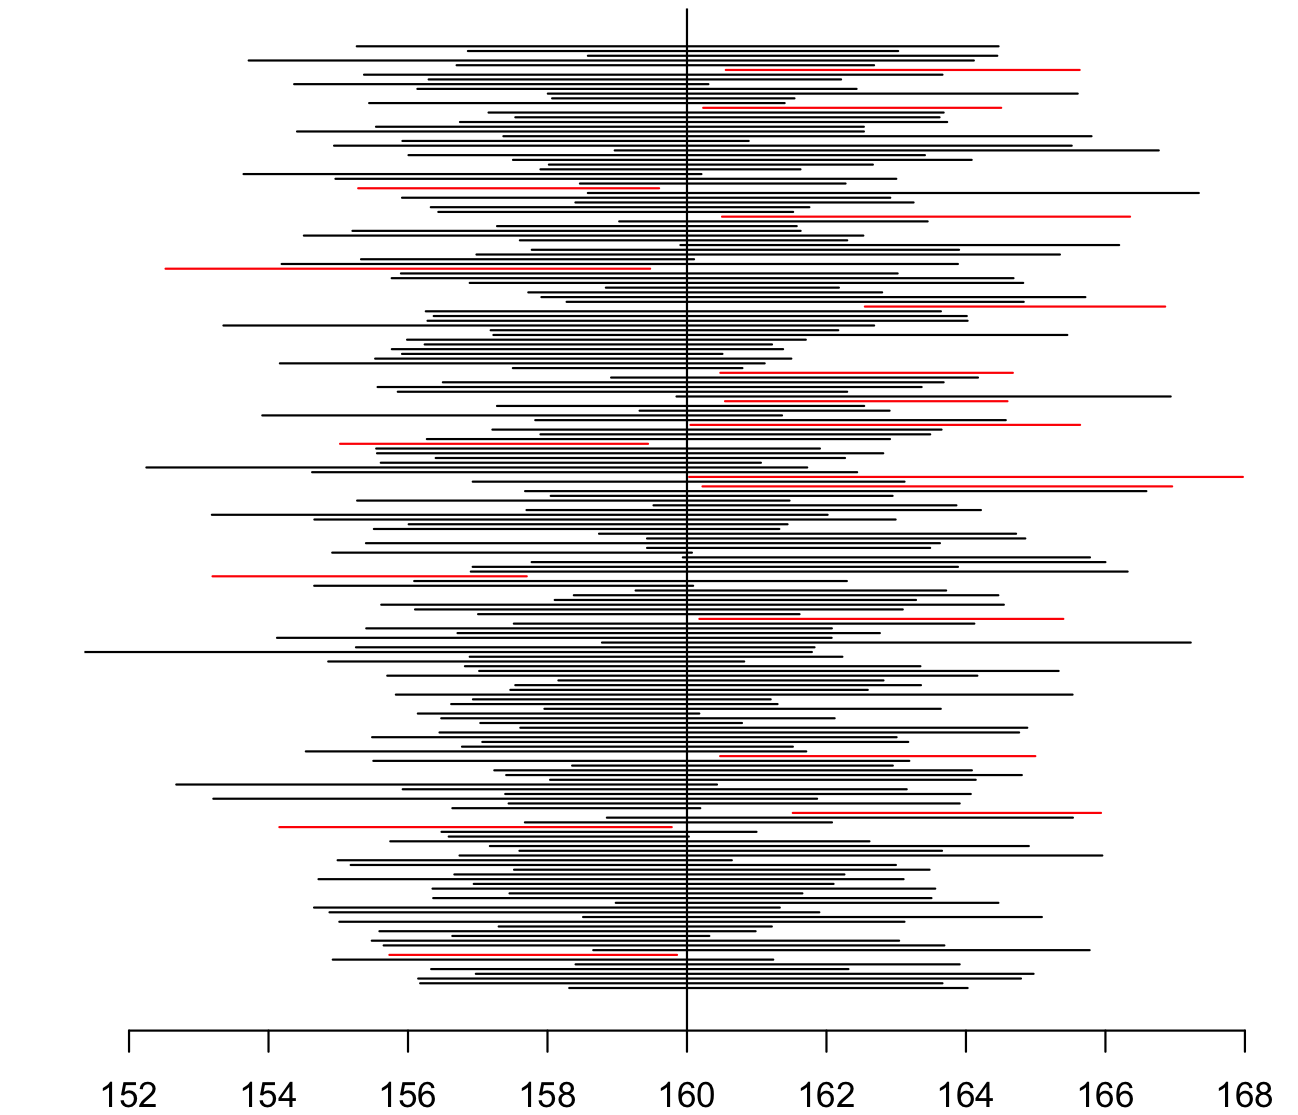
\includegraphics[width=0.8\textwidth]{figures/06-Confidence_interval/confidence_t.png}
        \caption{從 $\NN(160, 5^2)$ 抽出樣本數 9 的 200 組樣本所得的信賴區間（樣本標準差帶入母體標準差）}
        \label{fig:confidence_t}
    \end{figure}

    幸運的是，統計學家 William Gosset（1876—1937）在 1908 年提出了一個新的分布，能夠幫助我們找出在這個情境中精確建構信賴區間的方法。Gosset 提出，若母體服從平均值為 $\mu$ 的常態分布，並從中抽取樣本數為 $n$ 的樣本得到樣本平均 $\bar{X}$ 及樣本標準差 $s$，則
    \smallskip
    \[\frac{\bar{X}-\mu}{s/\sqrt{n}} \sim t_{n-1}\]
    \smallskip
    其中 $t_{n-1}$ 被稱為 student $t$ 分布（這裡如果 $t$ 能夠大寫代表隨機變數的確比較不容易混淆，但是統計學界的習慣都寫小寫）。下標的 $n-1$ 是 $t$ 分布唯一的參數，被稱為\textit{自由度} (degrees of freedom)。這個自由度的由來可以看成是分母在計算樣本標準差時，使用的樣本數減去估計的參數個數，因此是 $n$ 個樣本減掉估計了一個樣本平均，總自由度為 $n-1$。Gosset 當時所在的 Guinness 酒廠不允許他用本名發表該分布的論文，所以他使用了 student 這個化名（如圖 \ref{fig:student_biometrika} 所示），進而使 student 變成該分布的正式名稱。有興趣的讀者請參考以下\href{https://www.youtube.com/watch?v=qWDEzMgLbNY}{連結}。

    \begin{figure}[htbp]
        \centering
        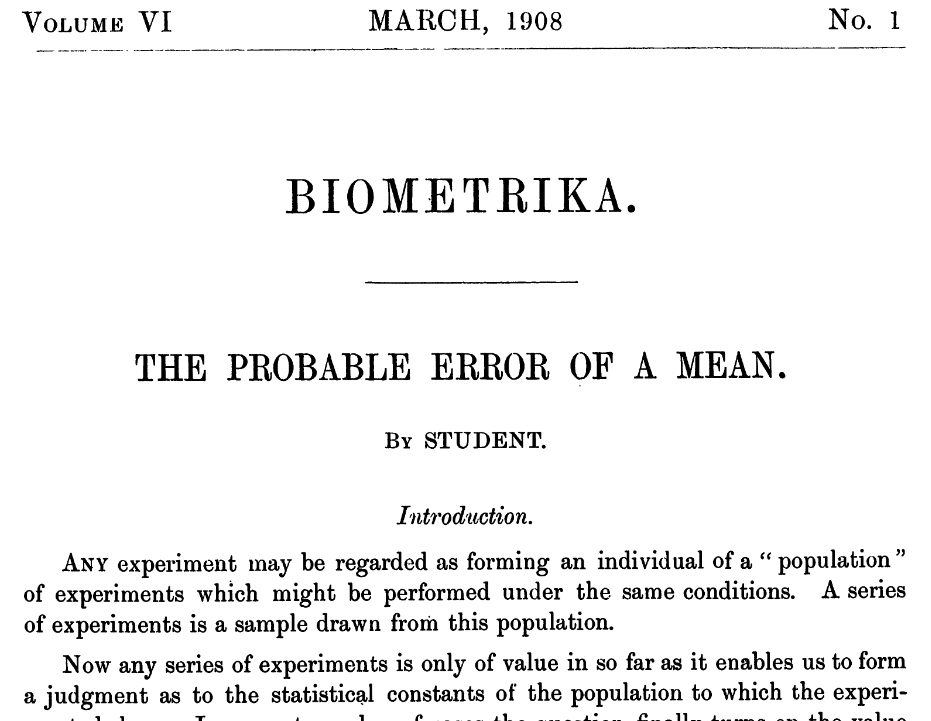
\includegraphics[width=0.6\textwidth]{figures/06-Confidence_interval/student_biometrika.png}
        \caption{William Gosset 有關 $t$ 分布的論文}
        \label{fig:student_biometrika}
    \end{figure}


    \medskip
    
    $t$ 分布的機率密度函數如圖\ref{fig:student}所示。可以看到相對於標準常態分布（黑色粗線） 而言，$t$ 分布的分布比較分散，雙尾比較厚重。但是隨著自由度 $\nu$ 上升，$t$ 分布的形狀會越來越接近標準常態分布。事實上，當自由度 $\nu > 30$ 時，一般認為 $t$ 分布可以直接用標準常態分布來近似。針對 $t$ 分布，我們也有 \href{https://en.wikipedia.org/wiki/Student%27s_t-distribution}{$t$分布表}可以查詢其曲線下面積。

    \begin{figure}[htbp]
        \centering
        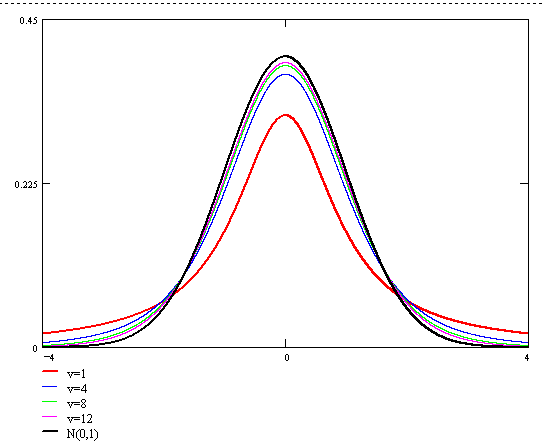
\includegraphics[trim={0 0 0 0.5cm},clip,width=0.7\textwidth]{figures/06-Confidence_interval/student.png}
        \caption{$t$分布的機率密度函數}
        \label{fig:student}
    \end{figure}

    回到我們建構信賴區間的目標，現在我們知道 $\frac{\bar{X}-\mu}{s/\sqrt{n}}$ 服從一個已知的 $t_{n-1}$ 分布，因此它又是一個樞紐量。我們可以參考前面的推導過程，先從以下的等式出發，針對 $t_{n-1}$ 建構出一個以 $0$ 為中心左右對稱，且機率為 $(1-\alpha)\times 100\%$ 的區間：
    \smallskip
     \[\PP(-t_{n-1, \alpha/2} < t_{n-1} < t_{n-1, \alpha/2}) = \alpha\]
    \smallskip
    其中 $t_{\nu, p}$ 代表滿足 $\PP(t_{\nu} > t_{\nu, p}) = p$的數值，可以用查表得到。根據前面的分布，我們可以推出：
    \smallskip
    \begin{align*}
        \PP\Big(-t_{n-1, \alpha/2} < \frac{\bar{X} - \mu}{s/\sqrt{n}} < t_{n-1, \alpha/2}\Big) &= \alpha\\
        \PP\Big(-t_{n-1, \alpha/2}\frac{s}{\sqrt{n}} < \bar{X} - \mu < t_{n-1, \alpha/2}\frac{s}{\sqrt{n}}\Big) &= \alpha\\
        \PP\Big(\bar{X}-t_{n-1, \alpha/2}\frac{s}{\sqrt{n}}< \mu < \bar{X} + t_{n-1, \alpha/2}\frac{s}{\sqrt{n}}\Big) &= \alpha\\
        \PP\Big(\mu \in \Big(\bar{X}-t_{n-1, \alpha/2}\frac{s}{\sqrt{n}},  \bar{X} + t_{n-1, \alpha/2}\frac{s}{\sqrt{n}}\Big)\Big) &= \alpha
    \end{align*}
    \smallskip
    因此，母體為常態分布下的母體平均值 $(1-\alpha)\times 100\%$ 信賴區間可以寫為
    \[\Big(\bar{X}-t_{n-1, \alpha/2}\frac{s}{\sqrt{n}},  \bar{X} + t_{n-1, \alpha/2}\frac{s}{\sqrt{n}}\Big)\]
    可以看到，用 $t$ 分布建構的信賴區間和常態分布建構的信賴區間，基本上只差在臨界值改成查 $t_{n-1}$ 的表、以及標準差由母體標準差改為樣本標準差。前面我們提到 $t$ 分布都比標準常態分布來得寬，所以 $t_{n-1, \alpha/2}$ 會比 $z_{\alpha/2}$ 來得大，也就是 $t$ 分布建構的信賴區間比常態分布建構的信賴區間來得寬。用類似的推導也可以得到右尾和左尾的 $(1-\alpha)\times 100\%$ 信賴區間分別可以寫為
    \[\Big(-\infty,  \bar{X} + t_{n-1, \alpha}\frac{s}{\sqrt{n}}\Big), \;\;\Big(\bar{X}-t_{n-1, \alpha}\frac{s}{\sqrt{n}},  \infty\Big)\]

    \bigskip

    \begin{custom}{動手作}
        假設已知 60 歲以上國人血清低密度脂蛋白的濃度呈現常態分布。現隨機選取 16 位 60 歲以上的志願者抽血，得到血清低密度脂蛋白的平均濃度為 93 mg/dL，樣本標準差為 9 mg/dL。請問 60 歲以上國人平均血清低密度脂蛋白濃度的 (1) 雙尾 95\% 信賴區間為何？ (2) 右尾 90\% 信賴區間為何？
    \end{custom}

    \answerbox{300pt}

    \begin{takehome}
        \item 區間估計同時提供未知參數的近似位置與不確定性。
        \item $(1-\alpha) \times 100\%$ 信賴區間以機率 $(1-\alpha) \times 100\%$ 覆蓋感興趣的參數，其變動性存在於區間而非參數上。
        \item $t$ 分布有一個參數，即自由度 $\nu$。
        \begin{itemize}
            \item 當自由度較小時，$t$ 分布的尾巴比標準常態分布來得厚
            \item 當自由度增大（例如，$>30$）時，$t$ 分布趨近於標準常態分布
        \end{itemize}
        \item 當母體服從常態分布時，母體平均的雙側\textit{精確} $(1-\alpha) \times 100\%$ 信賴區間為
        \[\Bigg(\bar{X} - t_{n-1, \alpha/2} \frac{s}{\sqrt{n}}, \bar{X} + t_{n-1, \alpha/2} \frac{s}{\sqrt{n}}\Bigg)\]
        \item 當母體不服從常態分布但樣本數較大時，母體平均的雙側\textit{近似} $(1-\alpha) \times 100\%$ 信賴區間可建構為
        \[\Bigg(\bar{X} - z_{\alpha/2} \sqrt{\frac{\hat{\sigma}^2}{n}}, \bar{X} + z_{\alpha/2} \sqrt{\frac{\hat{\sigma}^2}{n}}\Bigg)\]
        其中 $\hat{\sigma}^2$ 為母體變異數的估計量。
    \end{takehome}

    \bigskip
    
    \begin{docexam}{（107-1醫學(二)）}
        為了探討某社區之吸菸盛行狀況，由此社區隨機選取100位居民，發現其中30位居民具有吸菸習慣。在 5\% 的誤差水準下，此社區吸菸率的 95\% 信賴區間之上限值為何？
    \end{docexam} 
    
    \begin{docexam}{（103-1醫學(一)）}
        對 100 名國小六年級學童量測體重，發現樣本平均值為 35 公斤，母群體平均值的 95\% 信賴區間為 33 公斤至 37 公斤。下列敘述何者正確？

        (A) 母群體平均值為 35 公斤

        (B) 該研究 100 名國小學童中，95 名的體重介在 33 至 37 公斤之間

        (C) 該樣本學童的體重標準差約 10 公斤

        (D) 若計算母群體平均值的 90 \% 信賴區間，其範圍會大於 95\% 信賴區間
    \end{docexam}